% ======================================================
% Compile: xelatex 5state_aprime_coupdate.tex
% Path:    reference/eq17_analysis/derivation/5state_aprime_coupdate.tex
% DRAFT (2026-07-20, rev). CO-UPDATE a' update: a' is a KF state driven by BOTH
% (i) the var-ratio readout a'_hdm via a beta-EWMA (esti bolt-on, kept inside
% the estimator: sigma2_ar, sigma2_dhr, a'_hdm all computed) AND (ii) the KF
% innovation correction L51*e_y1 + L52*e_y2. Style/route follow
% 5state_aprime_var_esti.tex: 0 Def / 1 True (beta appears here) / 2 a'_hdm /
% 3 Esti (co-update) / 4 Error / 5 F_e / 6 Q,R / 7 Simulation.
% Extended (2026-07-21): 8.1 rewritten in math and MERGED with the first-hold
% oscillation (unobservable a' -> wander -> poisons a_hat_z via predict injection
% + Q44); 8.2 in math (a_d-state / kfmeas + C2 channel). A dither section was
% drafted and REMOVED -- the pilot confirmed dither's a'-Fisher scaling law but
% showed it does NOT clean a_hat_z (decoupled from the downstream a_xm floor).
% ======================================================
\documentclass[11pt,a4paper,fontset=none]{ctexart}

\usepackage[fleqn]{amsmath}
\usepackage{amssymb,bm}
\usepackage{empheq}
\setlength{\mathindent}{0pt}
\usepackage{geometry}
\geometry{margin=2.1cm}
\usepackage{array,booktabs}
\usepackage{graphicx}
\usepackage{xcolor}

\setlength{\parindent}{0pt}
\setlength{\parskip}{0.8em}
\setlength{\abovedisplayskip}{10pt}
\setlength{\belowdisplayskip}{10pt}
\setlength{\abovedisplayshortskip}{6pt}
\setlength{\belowdisplayshortskip}{6pt}

\newcommand{\lc}{\lambda_c}
\newcommand{\ap}{a'_{hd}}
\newcommand{\aph}{\hat a'_{hd}}
\newcommand{\apm}{a'_{hdm}}
\newcommand{\apmh}{\hat a'_{hdm}}
\newcommand{\dxh}{\delta\hat h}
% Section header with a one-line italic subtitle for readability
\newcommand{\hd}[2]{\par\medskip\noindent%
  \underline{\textbf{#1}}\quad{\small\itshape #2}\par\nobreak\vspace{0.4ex}}

\begin{document}

% ------------------------------------------------------------------
\hd{0. Definitions}{coordinates, the slope $\ap$, and the closed-loop tracking error}

\[
h[k] = h_d[k] - \delta h[k], \qquad
\Delta h_d[k] = h_d[k+1] - h_d[k]
\]
\[
\ap[k] := \left.\frac{d a_h}{d h}\right|_{h_d[k]}, \qquad
a_r[k] := a_h[k] - a_h\big(h_d[k]\big)
\]
\[
\delta h[k+1] = \lc\,\delta h[k] - F_{dh}[k]\,e_{a_h}[k] - \varepsilon_h[k]
\]

\begin{quote}\small
$a_h$ = actual-height gain (state 4); $\ap$ = its slope (state 5);
$a_r$ = residual gain from the tracking error.
$a_{var}=a_{cov}=0.05$ (EWMA weights);
$\beta = 1-T_s/\tau$ ($\tau=0.35$\,s $\Rightarrow \beta=0.99821$) = the $a'$
smoothing weight. $\delta h_1:=\delta h[k-d]$.
\end{quote}

% ------------------------------------------------------------------
\hd{1. True}{the residual is $-\ap\,\delta h$; hence the var-ratio recovers $\ap$, and the $\beta$-EWMA is its update law}

First-order Taylor of the gain at the perturbed height:
\[
a_h\big(h[k]\big) \approx a_h\big(h_d[k]\big) - \ap[k]\,\delta h[k]
\]
\begin{empheq}[box=\fbox]{equation*}
a_r[k] = -\,\ap[k]\,\delta h[k], \qquad \ap[k+1]\approx\ap[k]
\end{empheq}

Because the residual and the tracking error share the author $\ap$, their
variance ratio recovers the slope:
\[
\apm[k] := +\sqrt{\;\mathrm{Var}\big(a_r[k]\big)\,/\,\mathrm{Var}\big(\delta h[k]\big)\;}
= \ap[k] \qquad(\ap>0)
\]

The true update law for the slope is a $\beta$-EWMA of this readout --- consistent
because $\apm\equiv\ap$:
\begin{empheq}[box=\fbox]{equation*}
\ap[k+1] = \beta\,\ap[k] + (1-\beta)\,\apm[k], \qquad \apm \equiv \ap
\end{empheq}

% ------------------------------------------------------------------
\hd{2. $\apmh$}{the estimator's empirical var-ratio: two EWMA chains on $\hat a_h$ and $\dxh_3$}

Replace the true quantities by their estimates. One chain tracks the mean and
variance of the gain estimate, the other of the tracking-error estimate:
\[
\begin{aligned}
\overline a_h[k+1] &= (1-a_{var})\,\overline a_h[k] + a_{var}\,\hat a_h[k+1],
  & \hat a_r[k] &= \hat a_h[k] - \overline a_h[k] \\[1pt]
\hat\sigma^2_{\hat a_r}[k+1] &= (1-a_{cov})\,\hat\sigma^2_{\hat a_r}[k] + a_{cov}\,\hat a_r^2[k+1]
  & & \\[3pt]
\overline{\dxh}[k+1] &= (1-a_{var})\,\overline{\dxh}[k] + a_{var}\,\dxh_3[k+1],
  & \dxh_r[k] &= \dxh_3[k] - \overline{\dxh}[k] \\[1pt]
\hat\sigma^2_{\dxh}[k+1] &= (1-a_{cov})\,\hat\sigma^2_{\dxh}[k] + a_{cov}\,\dxh_r^2[k+1]
  & &
\end{aligned}
\]
\begin{empheq}[box=\fbox]{equation*}
\apmh[k] := +\sqrt{\;\hat\sigma^2_{\hat a_r}[k]\,\big/\,\hat\sigma^2_{\dxh}[k]\;}
\end{empheq}

% ------------------------------------------------------------------
\hd{3. Esti (co-update)}{$\ap$ is updated by the $\beta$-EWMA of $\apmh$ \emph{plus} the KF innovation correction}

State $\ x = [\,\delta h_1,\ \delta h_2,\ \delta h_3,\ a_h,\ \ap\,]^{\mathsf T}$.
The KF proper corrects $[\delta h_1,\delta h_2,\delta h_3,a_h]$ from $y_1=\delta x_m$
and $y_2=a_{xm}$; innovations $e_{y_1}=y_1-\hat y_1$, $e_{y_2}=y_2-\hat y_2$;
gain $K=P^-H^{\mathsf T}S^{-1}$, $S=HP^-H^{\mathsf T}+R$.

\[
\hat a_h[k+1] = \hat a_h[k] + \aph[k]\big(\Delta h_d[k] + (1-\lc)\,\dxh_3[k]\big)
\qquad(\text{gain-level predict})
\]

\begin{empheq}[box=\fbox]{equation*}
\aph[k+1] =
\underbrace{\beta\,\aph[k] + (1-\beta)\,\apmh[k]}_{\text{(i) var-ratio }\beta\text{-EWMA (\S1 form)}}
\;+\;
\underbrace{L_{51}[k]\,e_{y_1}[k] + L_{52}[k]\,e_{y_2}[k]}_{\text{(ii) KF }L\cdot e\text{ correction}}
\end{empheq}

\begin{quote}\small
$L_{5j}=[P^-H^{\mathsf T}S^{-1}]_{5,j}$. With $H(\cdot,5)=0$ (no own measurement
row for $\ap$), $L_{5j}$ is a \emph{cross-covariance} gain
$\propto P^-_{5,4}\,H(j,4)$, built by the coupling $F_e(4,5)=\Delta h_d$.
Setting $L\!\cdot\!e=0$ recovers the pure esti bolt-on; dropping $(1-\beta)\apmh$
recovers the pure as-state.
\end{quote}

% ------------------------------------------------------------------
\hd{4. Error}{how the estimate errors evolve}

$e_{a_h}=a_h-\hat a_h$, \ $e_{\ap}=\ap-\aph$, \ $e_h=\delta h-\dxh$.
\[
e_{a_h}[k+1] = \big(1+\aph F_{dh}\big)\,e_{a_h}
+ \Delta h_d\,e_{\ap} + (1-\lc)\,\aph\,e_h + \aph\,\varepsilon_h
\]
\begin{empheq}[box=\fbox]{equation*}
e_{\ap}[k+1] = \beta\,e_{\ap}[k]
\;-\;(1-\beta)\big(\apmh[k]-\apm[k]\big)
\;-\;(\text{KF correction})
\end{empheq}
The middle term is the var-ratio readout error (self-copy $+$ noise); the last is
the genuine measurement pull --- the $L\!\cdot\!e$ term of \S3, kept symbolic here.

% ------------------------------------------------------------------
\hd{5. $\mathbf F_e$ and $\mathbf H$}{the $5\times5$ transition and $2\times5$ measurement Jacobians}

\[
F_e[k] =
\begin{bmatrix}
0 & 1 & 0 & 0 & 0 \\[1pt]
0 & 0 & 1 & 0 & 0 \\[1pt]
0 & 0 & \lc & -F_{dh}[k] & 0 \\[1pt]
0 & 0 & (1-\lc)\aph[k] & 1+\aph[k]F_{dh}[k] & \Delta h_d[k] \\[1pt]
0 & 0 & 0 & 0 & \beta
\end{bmatrix},
\qquad
H =
\begin{bmatrix}
1 & 0 & 0 & 0 & 0 \\[1pt]
0 & 0 & 0 & 1 & 0
\end{bmatrix}
\]

\begin{quote}\small
Row-5 pole $=\beta$ (the EWMA memory); the $(1-\beta)\apmh$ drive and the
$L\!\cdot\!e$ correction enter as inputs, not through the pole.
$F_e(4,5)=\Delta h_d$ is the \emph{only} path giving $\ap$ a Kalman gain.
\end{quote}

% ------------------------------------------------------------------
\hd{6. $\mathbf Q$ and $\mathbf R$}{process and measurement noise}

\[
Q = \mathrm{diag}\big(0,\ 0,\ Q_{33},\ Q_{44},\ Q_{55}\big),
\qquad
R = \mathrm{diag}\big(\sigma^2_{n},\ R_2\big)
\]
\[
Q_{33} = 4k_BT\,\hat a_h\big(1+(1-\lc)^2 d\big) + (1-\lc)^2\sigma^2_{n},
\qquad
Q_{44} = \big(\hat a_h K_h/R\big)^2\,\sigma^2_{\delta h},
\qquad
Q_{55} = (1-\beta)^2\,R_{var}
\]
\[
R_2 = a_{cov}\,IF_{var}\,\big(\hat a_h+\xi\big)^2,
\qquad
R_{var}\approx \tfrac{a_{cov}}{4}\big(IF_{\hat a_r}+IF_{\dxh}-2IF_\times\big)\,\aph{}^{2}
\]

\begin{quote}\small
$\sigma^2_{\delta h}=4k_BT\,\hat a_h$;\ \
$\xi=(C_n/C_{dpmr})\,\sigma^2_n/(4k_BT)$;\ \
$IF_\ast=1+2\sum_{j\ge1}\rho_\ast(j)(1-a_{cov})^j$.
$Q_{55}$ is the injected variance of the $(1-\beta)\apmh$ drive.
\end{quote}

% ------------------------------------------------------------------
\hd{7. Simulation (1 Hz)}{co-update traces, init $1\times$}

\begin{center}
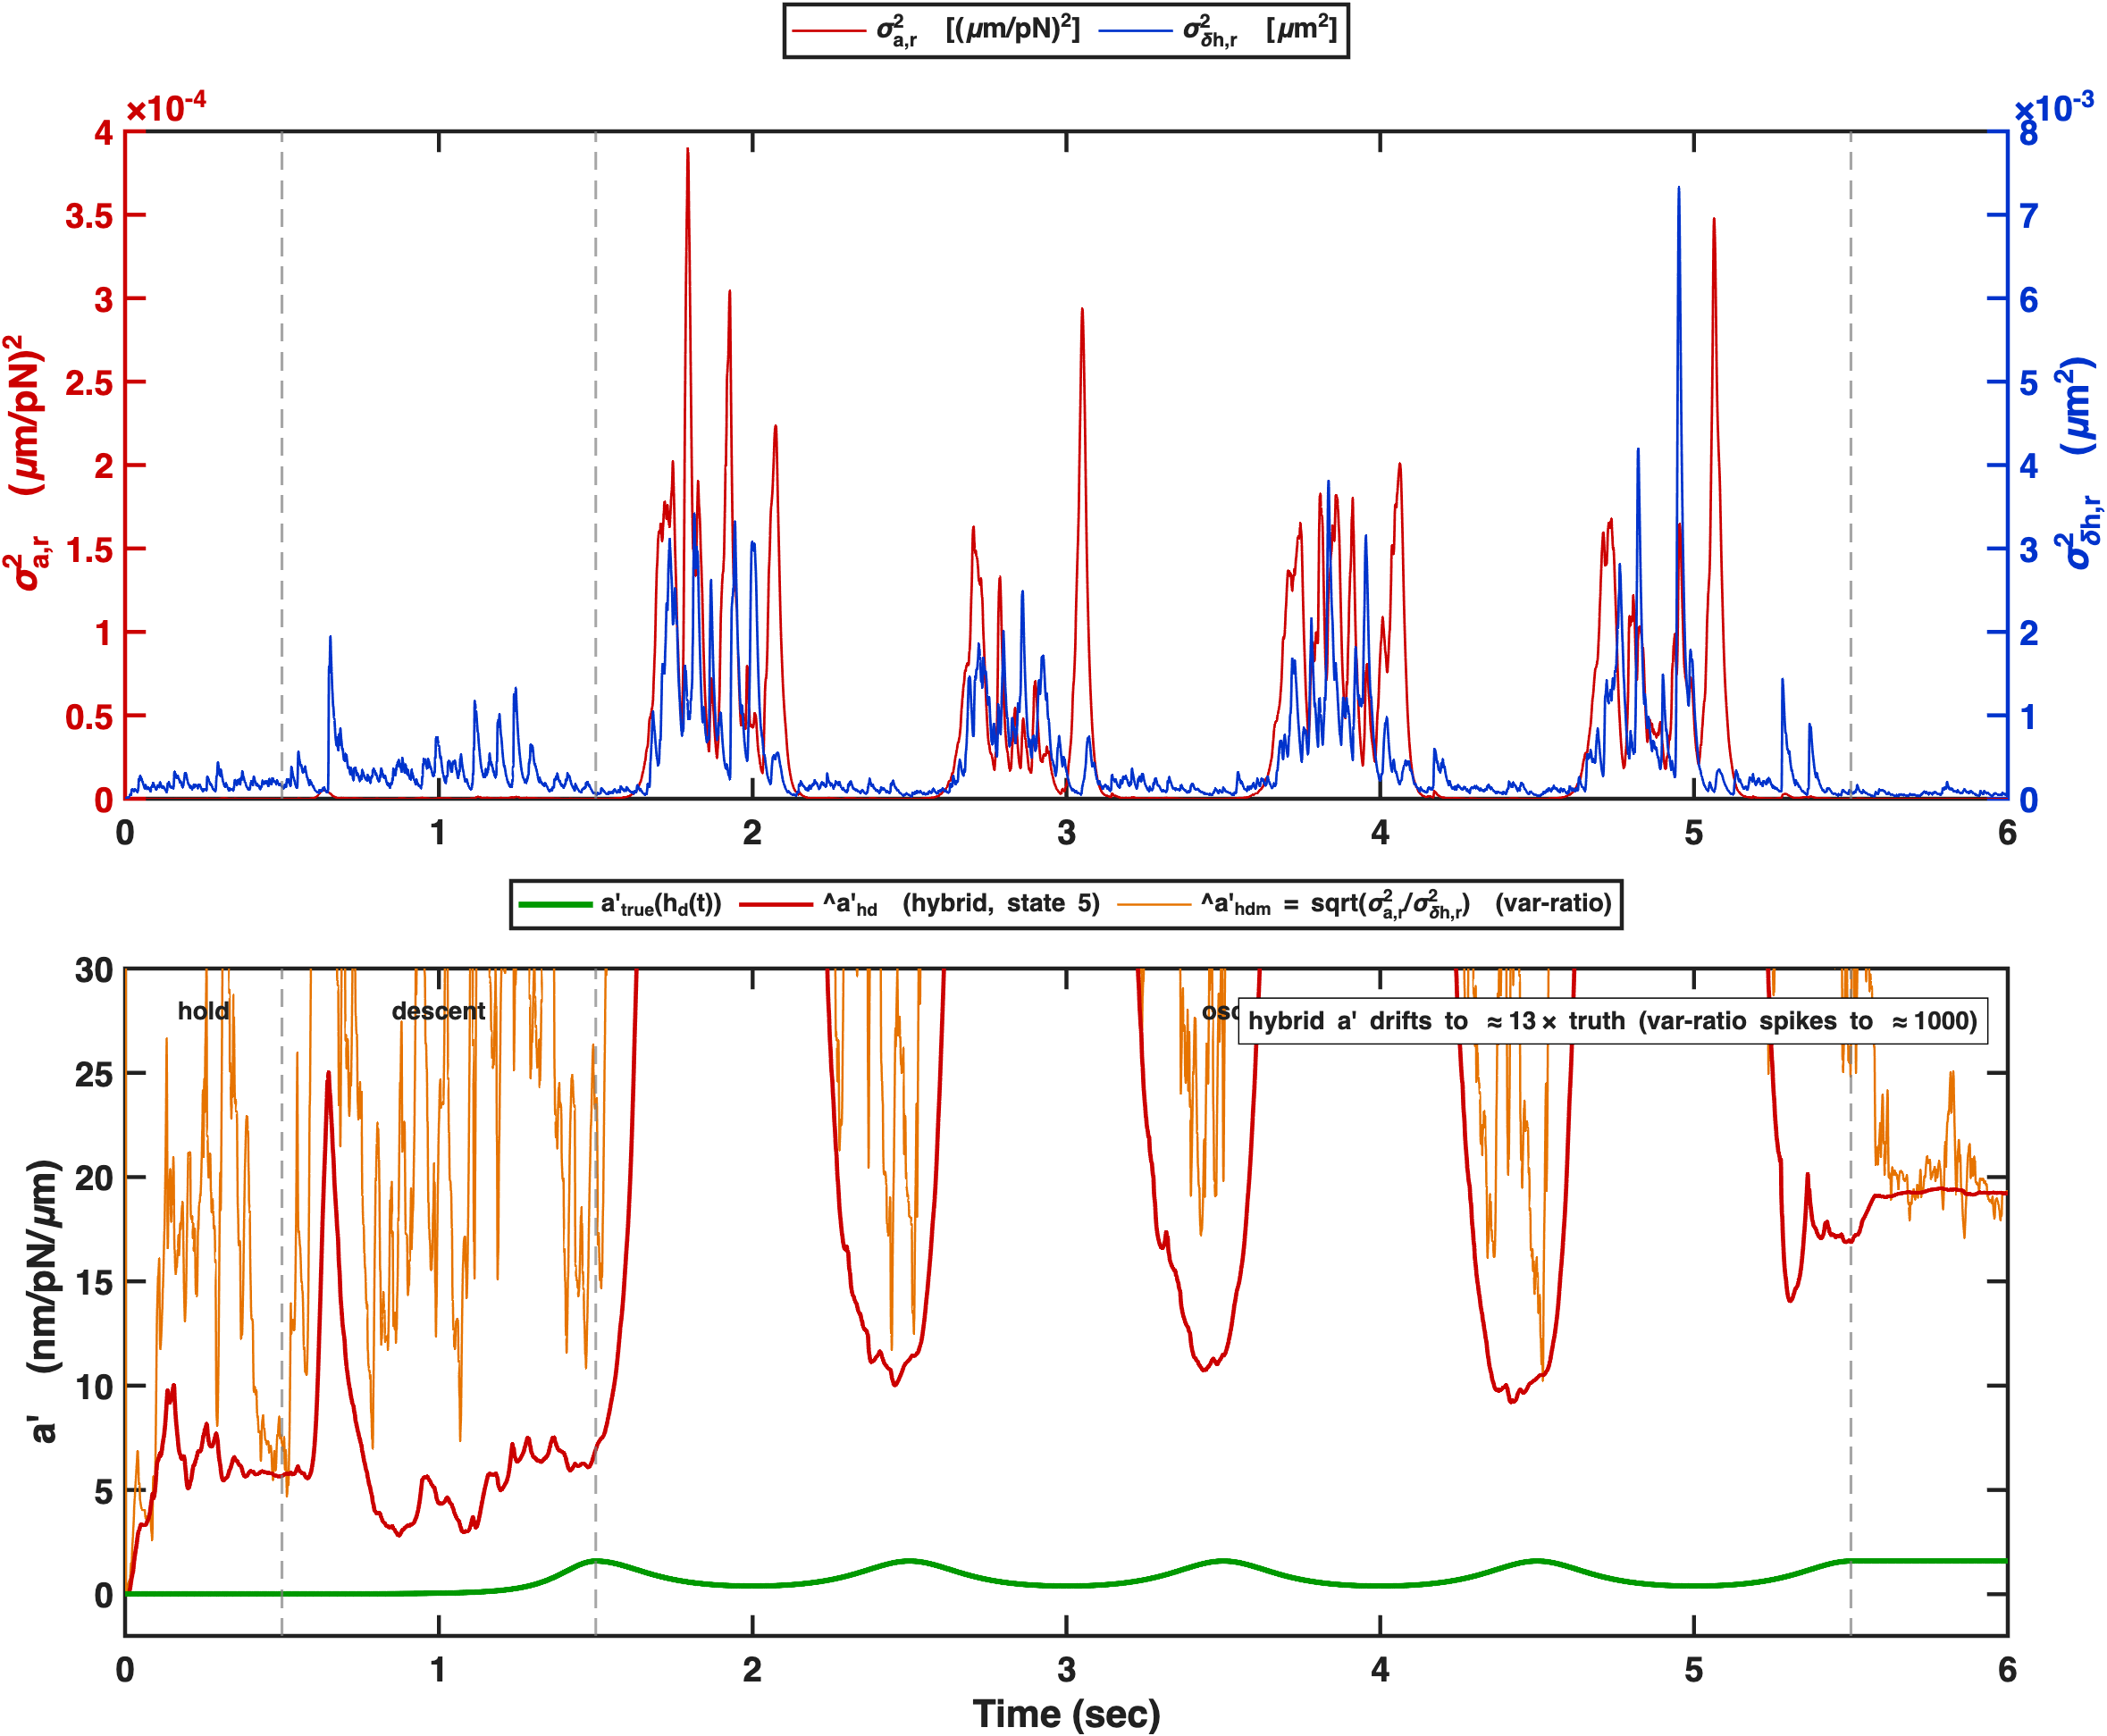
\includegraphics[width=0.90\textwidth]{figures/coupdate_var_aprime.png}
\end{center}

\begin{center}
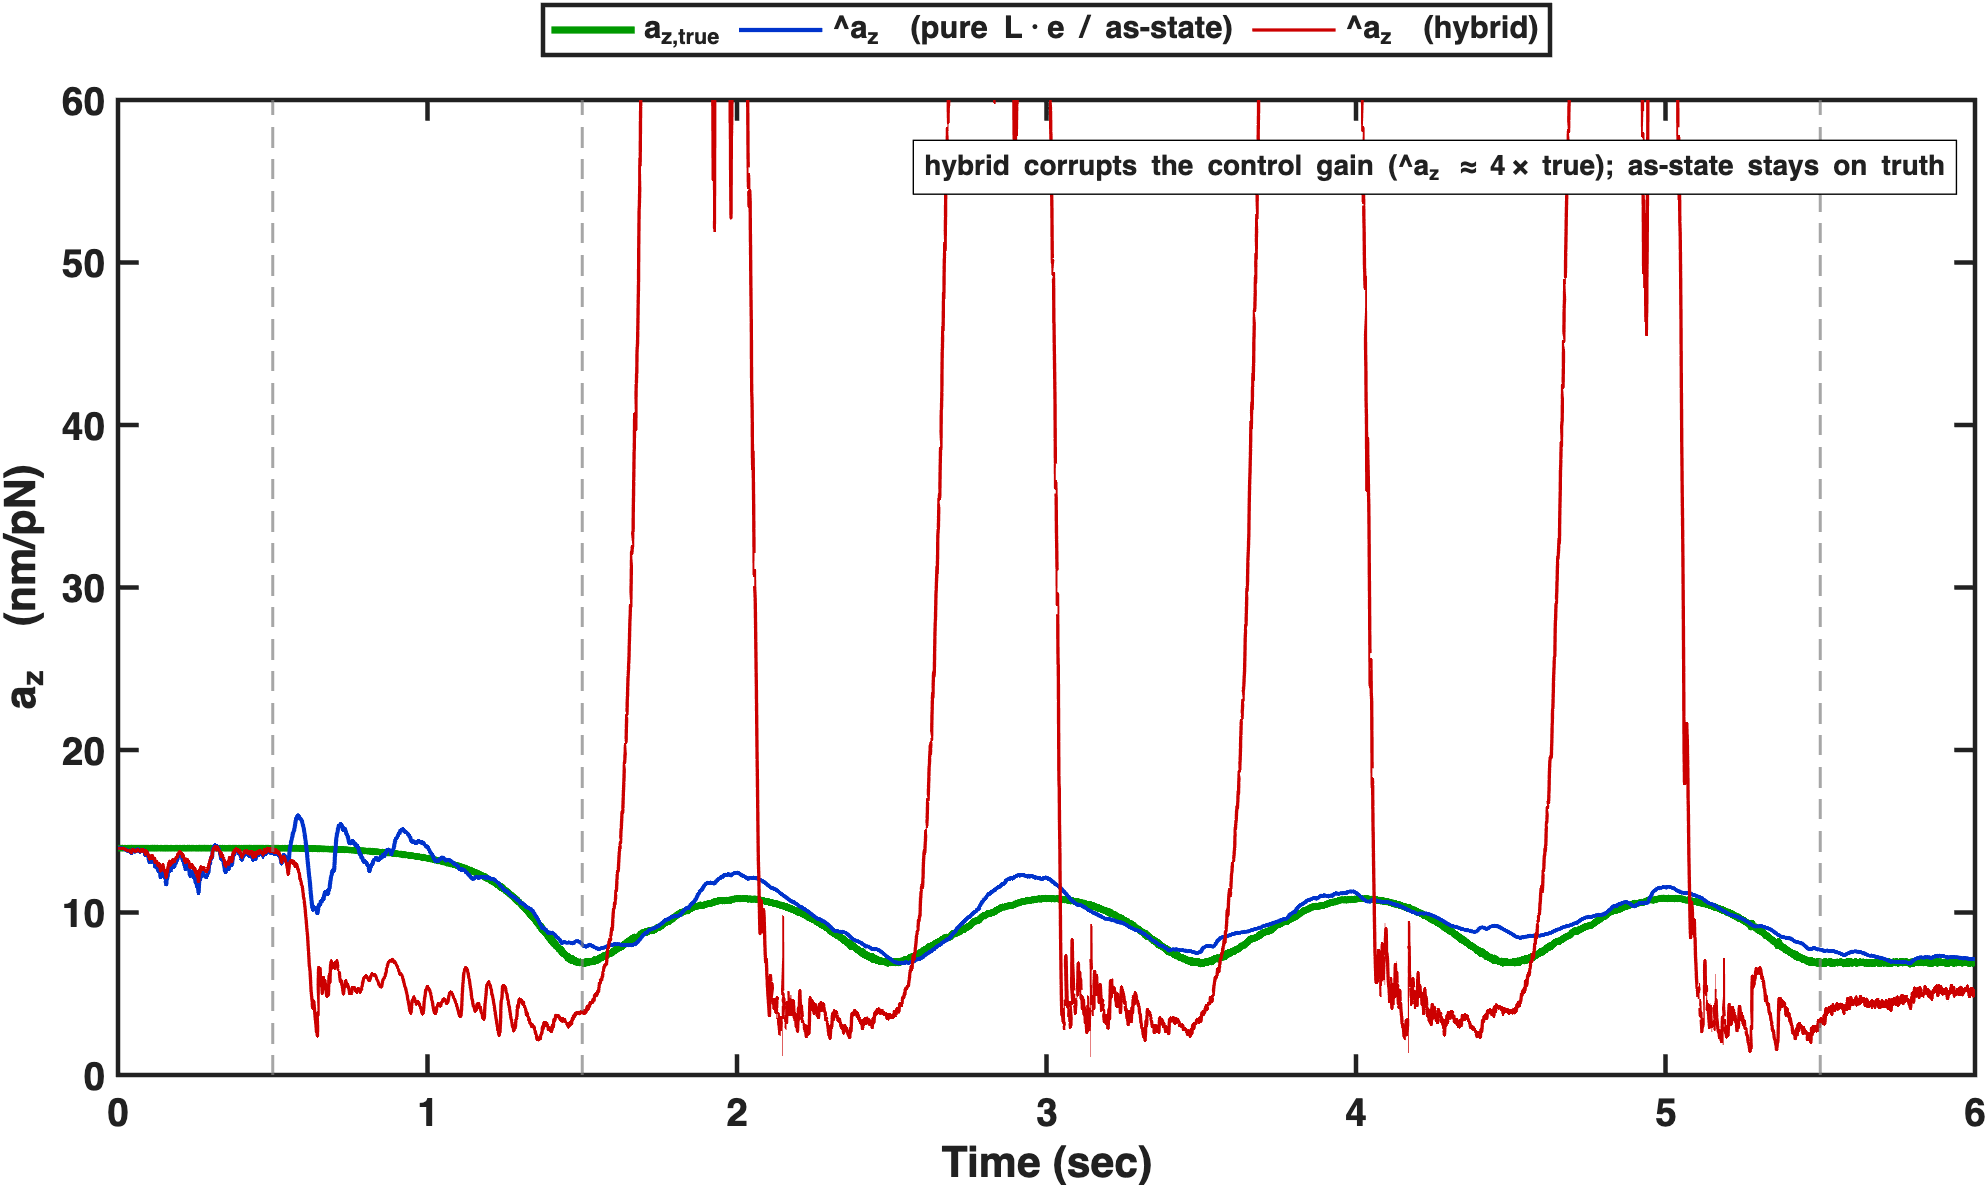
\includegraphics[width=0.90\textwidth]{figures/coupdate_ahat.png}
\end{center}

% ==================================================================
\hd{8. As-state (the blue line): drop the var-ratio}{$\ap$ is a plain KF state, corrected by $L\!\cdot\!e$ only --- no $\apmh$}

Start from the same True relation (\S1): $\ a_r[k]=-\ap[k]\,\delta h[k]$,
$\ \ap[k+1]\approx\ap[k]$. The as-state estimator keeps $\ap$ as a plain 5th KF
state and \emph{removes the var-ratio channel entirely} --- no $\apmh$, no
$\beta$-EWMA. State $\ x=[\,\delta h_1,\delta h_2,\delta h_3,a_h,\ap\,]^{\mathsf T}$.

\[
\text{Predict:}\quad
\hat a_h[k+1] = \hat a_h[k] + \aph\big(\Delta h_d + (1-\lc)\,\dxh_3\big),
\qquad
\aph[k+1] = \aph[k]\ \ (\text{integrator}).
\]

\begin{empheq}[box=\fbox]{equation*}
\text{Update (KF only):}\qquad
\aph[k+1] = \aph[k] + L_{51}\,e_{y_1} + L_{52}\,e_{y_2}
\end{empheq}

With $H=\big[\begin{smallmatrix}1&0&0&0&0\\ 0&0&0&1&0\end{smallmatrix}\big]$
($H(\cdot,5)=0$), $L_{5j}$ is a \emph{cross-covariance} gain
$\propto P^-_{5,4}$, built solely by $F_e(4,5)=\Delta h_d$:
\[
F_e[k] =
\begin{bmatrix}
0 & 1 & 0 & 0 & 0 \\[1pt]
0 & 0 & 1 & 0 & 0 \\[1pt]
0 & 0 & \lc & -F_{dh} & 0 \\[1pt]
0 & 0 & (1-\lc)\aph & 1+\aph F_{dh} & \Delta h_d \\[1pt]
0 & 0 & 0 & 0 & 1
\end{bmatrix},
\qquad
Q_{55} = \sigma^2_{a''}\big(\Delta h_d^2 + \sigma^2_{\delta h}\big).
\]

\begin{quote}\small
Row-5 pole $=1$ (pure integrator, cf.\ $\beta$ in the co-update); $\ap$ moves
\emph{only} through the $L\!\cdot\!e$ correction. $\sigma^2_{a''}\sim(a_{nom}/R^2)^2$
is the sole curvature prior. This is the blue line: $\hat a_z$ on truth
($1.04\times$), tracking $26.5$ nm; $\ap$ underestimated in holds
($\Delta h_d\to0$, cross-cov gain $\to0$ --- the hold-desert CRLB floor).
\end{quote}

\medskip
\hd{8.1 $\hat a_z$ jitter, and its first-hold amplification when $\ap$ is unobservable}{a leak-free gain integrator; the sole measurement $a_{xm}$ sets a floor that an unobservable $\ap$ exceeds}

Gain: a leak-free integrator, one noisy measurement, two $\aph$-driven inputs:
\[
F_e(4,4)\approx1,\qquad \text{measurement } y_2=a_{xm}\ (\text{rel.\ std }0.37\text{--}0.54),
\]
\[
\hat a_z[k{+}1]=\hat a_z[k]+\underbrace{(1{-}\lc)\,\aph\,\dxh_3[k]}_{\text{(B) predict injection}}+\cdots,
\qquad
\underbrace{Q_{44}=\aph{}^{2}Q_{33}}_{\text{(Q) process noise}} .
\]

$\ap$ enters $y_2$ \emph{only} through the gain, with regressor $\varphi$; hence its Fisher information and CRLB:
\[
\varphi[k]:=\Delta h_d[k]+(1-\lc)\dxh_3[k],\qquad e_{a_h}[k{+}1]\supset\varphi[k]\,e_{\ap}[k],
\]
\[
\mathcal I(\ap)=\frac{1}{S_2}\sum_k\varphi^2[k],\qquad \mathrm{Var}(\aph)\ge\mathcal I^{-1}(\ap)\qquad(\text{CRLB}).
\]
\begin{empheq}[box=\fbox]{equation*}
\text{far hold: }\Delta h_d=0\Rightarrow \varphi=(1{-}\lc)\dxh_3\Rightarrow \mathcal I(\ap)\!\to\!0\Rightarrow \aph\ \text{drifts}\ (\aph\!\to\!6\text{--}13\ \text{vs}\ \ap\!\approx\!0)
\end{empheq}

The drifting $\aph$ drives both inputs; the gain jitter scales with them:
\[
\text{(B): } \sigma_{\rm inj}=(1{-}\lc)\,|e_{\ap}|\,\sigma_{\delta h}\ /\text{step};
\qquad
\text{(Q): } P_{44}\!\propto\!Q_{44}\!\propto\!\aph{}^{2}\Rightarrow L_4\!\propto\!P_{44}\Rightarrow \mathrm{Var}(\hat a_z)|_{\rm meas}\!\sim\!L_4^2R_2 .
\]
\begin{empheq}[box=\fbox]{equation*}
\aph\!\to\!0\Rightarrow\text{(B),(Q)}\!\to\!0\Rightarrow \mathrm{std}(\hat a_z)=0.015;
\qquad
\aph\ \text{drifting}\Rightarrow \mathrm{std}(\hat a_z)=0.61\ (40\times).
\end{empheq}

The $\sim\!5\%$ far-wall hold jitter ($\langle|\hat a_z-a_z|\rangle=0.73$ nm/pN) is thus the \emph{removable} $\aph$-drift, not the $a_{xm}$ floor ($0.015$, frozen $\aph$). First-hold fix: disable the $\aph$-update where $\mathcal I(\ap)\!\to\!0$ (freeze during the hold, resume at the first motion); accurate-$\hat a_z$ levers in \S8.2.

\medskip
\hd{8.2 Two charter-legal fixes for accurate $\hat a_z$}{(a) a reverting $a_d$-state removes the drift; (b) an independent $c$-free channel $C_2$ passes the $a_{xm}$ floor}

Charter: $c(\bar h)$ unknown; only $a_{nom},R,T_s$, wall position, commanded trajectory usable.

\textbf{(a) $a_d$-state (\texttt{kfmeas}): reversion, not a free integrator.}
\[
a_d:=a_h(h_d)\ (\text{desired-height gain}),\qquad
a_d[k{+}1]=a_d[k]+\aph\,\Delta h_d[k]\ \ (\text{deterministic, exogenous}) .
\]
\begin{empheq}[box=\fbox]{equation*}
\hat a_z=a_d-\aph\,\dxh_3;\qquad
\text{predict-side drift }2.74\%\to0.09\%\ (\sim30\times),\ \text{no }c(\bar h) .
\end{empheq}

\textbf{(b) $C_2$: a second gain channel, independent of $a_{xm}$.}
A gain error produces a \emph{systematic} tracking residual:
\[
f_d=\tfrac{1}{\hat a}\{\cdots\}
\ \Rightarrow\
\delta x_{md}\ \propto\ \frac{a-\hat a}{\hat a},
\qquad
y_3:=\delta x_{md}\ (\text{deterministic residual, } =p_{md}) .
\]
\begin{empheq}[box=\fbox]{equation*}
\mathbb E[y_3]=\kappa_{C_2}\,(a-\hat a),\quad \kappa_{C_2}\approx0.90\text{--}0.94\ (\text{unbiased, }c\text{-free}),\quad \text{floor}\sim9.4\%\,a/0.5\text{s} .
\end{empheq}
$C_2$ measures the gain error directly, independent of $a_{xm}$; $a_{cov}/Q_{44}/R_2$ tuning only trades jitter for lag and cannot pass the $a_{xm}$-only floor.

% ==================================================================
\hd{9. Appendix: the self-copy $\apmh\equiv\aph$ ($\kappa\approx0$)}{why the var-ratio carries no truth}

In a hold ($\Delta h_d=0$) the gain predict reduces to
$\ \hat a_h[k+1]=\hat a_h[k]+(1-\lc)\,\aph\,\dxh_3[k]$. Using the telescoping
identity $\ (1-\lc)\,\dxh_3[j]=\dxh_3[j]-\dxh_3[j+1]\ $ and summing from $k_0$,
\[
\hat a_h[k] = \hat a_h[k_0] + \aph\big(\dxh_3[k_0]-\dxh_3[k]\big)
\quad\Longrightarrow\quad
\hat a_r[k] = -\,\aph[k]\,\dxh_r[k].
\]
So $\hat a_r$ is built \emph{from} $\aph$, and the two variances are locked:
\[
\hat\sigma^2_{\hat a_r} = \aph{}^{2}\,\hat\sigma^2_{\dxh}
\]
\begin{empheq}[box=\fbox]{equation*}
\apmh = \sqrt{\;\hat\sigma^2_{\hat a_r}\big/\hat\sigma^2_{\dxh}\;} = \aph
\qquad\text{for \emph{any} true } \ap
\end{empheq}
The readout echoes the estimate, independent of the truth; its fidelity is
\[
\kappa := \frac{\partial\,\apmh}{\partial\,a'_{\mathrm{true}}} = 0.
\]
(The measured $\kappa\approx0.03$ and the $+2.5\%$ sqrt-rectification bias
$b_u\propto1/\aph$ come from the correction terms and finite EWMA windows; both
are $\ll1$, so the echo dominates.)

% ==================================================================
\hd{10. Appendix: the leak --- the motion face of the self-copy}{why the var-ratio is garbage in motion, and why the leak cannot be fixed}

In motion the gain estimate $\hat a_h$ swings to track the changing desired-height
gain $a_{\det}(t)$ (via the feedforward $\aph\,\Delta h_d$). The mean-tracker
$\overline a_h=\mathrm{EWMA}(\hat a_h)$ is a low-pass; its complementary high-pass
$\hat a_r=\hat a_h-\overline a_h$ does \emph{not} remove this swing fully --- it
leaks a fraction
\[
\lambda_{\mathrm{leak}} \approx \frac{2\pi f\,T_s}{a_{var}} \approx 0.079
\]
of it into $\hat a_r$. Since the deterministic swing ($\sim$nm/pN) dwarfs the
thermal residual $a_r=-\ap\,\delta h$ ($\sim0.04$ nm/pN), even a $7.9\%$ leak
dominates: $\sigma^2_{\hat a_r}$ inflates far above the thermal
$\aph{}^{2}\sigma^2_{\dxh}$, so
$\apmh=\sqrt{\sigma^2_{\hat a_r}/\sigma^2_{\dxh}}\gg\aph$.

\begin{center}
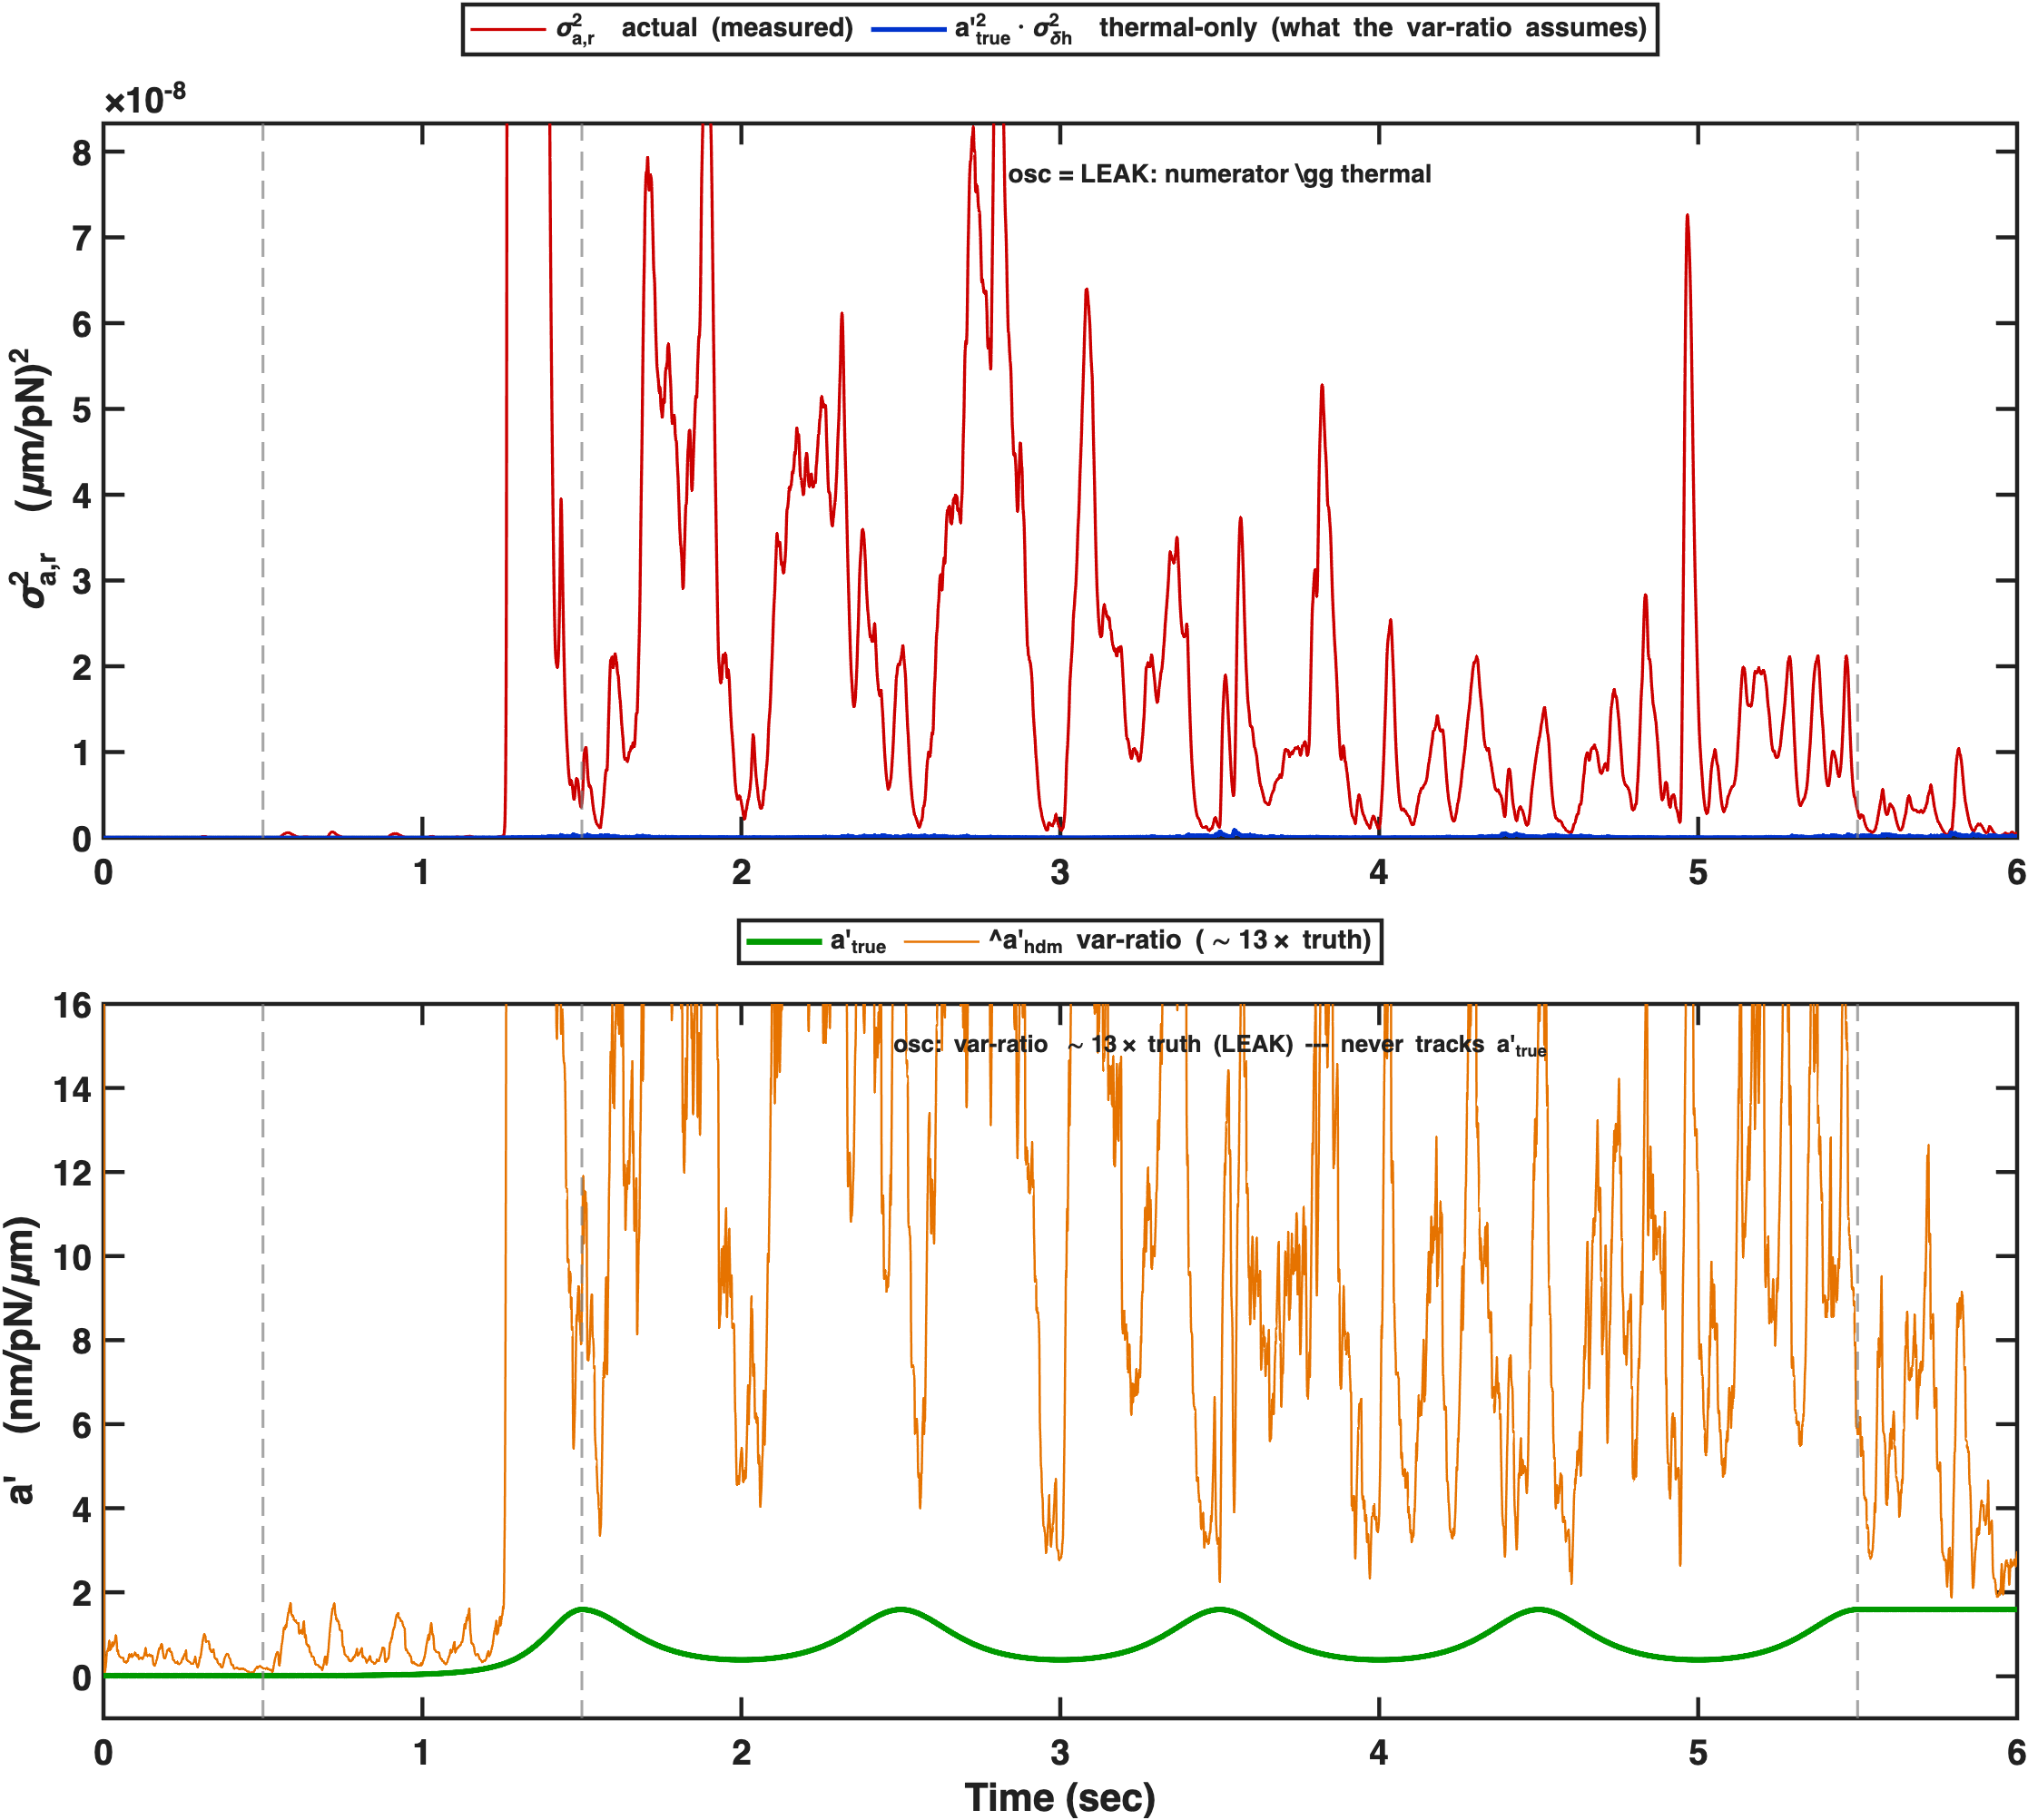
\includegraphics[width=0.90\textwidth]{figures/leak_mechanism.png}
\end{center}
\textit{Diagnostic var-ratio computed from a healthy as-state $\aph$. Top: the
actual numerator $\sigma^2_{a,r}$ (red) sits $\sim170\times$ above the thermal-only
value it should have (blue) during osc --- the leak. Bottom: the var-ratio
$\apmh$ (orange) is $\sim13\times$ truth (green) --- garbage --- during motion, and
never tracks $a'_{\mathrm{true}}$.}

\medskip
\textbf{Why it cannot be fixed.} The leaked swing is itself $\aph$-driven (the
feedforward uses $\aph$), so $\apmh$ stays $\aph$-derived --- the leak is the
\emph{motion} face of the same self-copy whose \emph{hold} face is \S9's echo.
Removing the leak (faster mean-tracker, or subtracting the feedforward) only turns
motion-garbage back into the hold echo $\apmh\equiv\aph$ --- still no truth; the
root ($\hat a_r$ built from $\aph$) is untouched. The clean fix is not to repair
the var-ratio but to drop it (pure $L\!\cdot\!e$ / as-state, or
\texttt{5state\_aprime\_kf\_meas}).

\end{document}
